\documentclass[12pt,a4paper]{article}

% Packages
\usepackage[utf8]{inputenc}
\usepackage{amsmath}
\usepackage{amsfonts}
\usepackage{amssymb}
\usepackage{graphicx}
\usepackage{hyperref}
\usepackage{algorithm}
\usepackage{algpseudocode}
\usepackage{booktabs}
\usepackage{listings}
\usepackage{enumerate}
\usepackage{pythontex}
\usepackage{lstmisc}
\usepackage{subcaption}


\usepackage{tikz}
\usepackage{xcolor}
\usepackage{siunitx}
\usepackage{float}
\usepackage{cleveref}

% Document settings
\title{Sudoku Forschungsprojekt Dokumentation}
\author{Bastian Fischer, Samuel Jaschke, Hannes Träger, Paul Volk}
\date{\today}

\begin{document}

\maketitle

\begin{abstract}
\end{abstract}

\section{Einleitung}
Der folgende Abschnitt beschreibt die Motivation und die grundlegenden Ziele des Projekts.

\subsection{Motivation}
Als Motivation diente ein Sudoku-Heft mit bestimmten partiellen Sudokus,
welche ”Bilder” von Katzen darstellen.
Die Idee war, ein Programm zu entwickeln, mit welchem man solche Sudokus generieren kann.

\subsection{Ziele}
Das Ziel des Projekts ist die Bereitstellung eines grafischen Benutzer-Interfaces (GUI) für das Erstellen
von partiellen Sudoku’s mit vorgegebenen Zellen, welche ein bestimmtes Muster erzeugen.
Außerdem soll es möglich sein für einige dieser Zellen explizit Ziffern festzulegen.
Des weiteren soll für ein partielles Sudoku dessen Schwierigkeit abgeschätzt werden können.

\subsection{Aufbau}
In \cref{sec:theoretische_ueberlegungen} werden einige theoretischen Vorüberlegungen zu Sudokus angestellt.
Anschließend wird in \cref{sec:backend} das Backend beschrieben.
Das Backend ist zum einen für die Generierung von partiellen Sudokus zuständig,
zum anderen für das Lösen von Sudokus und für die Bewertung der Schwierigkeit.
Den Abschluss bilden die Abschnitte \cref{sec:frontend} und \cref{sec:kommunikation},
welche vom Frontend und der Kommunikation zwischen Frontend und Backend handeln.



\section{Theoretische Überlegungen}
\label{sec:theoretische_ueberlegungen}

\input{Sections/TheoretischeÜberlegungen.tex}

\section{Backend}
\label{sec:backend}
Um die partiellen Sudokus zu erstellen, auf Eindeutigkeit zu überprüfen und die Schwierigkeit zu bewerten,
werden immer wieder folgende Schritte durchlaufen:
\begin{enumerate}
    \item \label{step:fill} Markierte Felder mit Ziffern füllen
    \item \label{step:unique} Partielles Sudoku auf Eindeutigkeit überprüfen
    \item \label{step:permute} Permutation der Ziffern im partiellen Sudoku
    \item \label{step:difficulty} Bewertung des Schwierigkeitsgrads des partiellen Sudokus
\end{enumerate}
Für den Modus, wo nur Zahlen gegeben sind, werden die Schritte~\ref{step:fill} und~\ref{step:permute} weggelassen.
Für die Modi, wo Felder markiert werden, auf wenn einzelne Ziffern gesetzt werden, werden alle Schritte durchlaufen.
Die genaue Ausführung der Schritte unterscheidet sich lediglich in Schritt~\ref{step:permute}.
Wenn Schritt~\ref{step:unique} fehlschlägt, das heißt das Sudoku entweder nicht lösbar ist oder mehrere Lösungen hat,
wird Schritt~\ref{step:fill} wiederholt, bis ein valides partielles Sudoku gefunden wurde.

\subsection{Markierte Felder befüllen}
Für die Befüllung der markierten Felder haben wir verschiedene Ansätze ausprobiert.

\subsubsection{Backtracking}
Der erste Ansatz war ein Backtracking-Algorithmus, der rekursiv versucht, die markierten Felder mit Ziffern zu füllen.
Wenn wir eine Belegung gefunden haben, die allerdings nicht lösbar oder mehrdeutig war, haben wir den Algorithmus weiterlaufen lassen,
bis eine eindeutige Lösung gefunden wurde, oder eine maximale Anzahl an Versuchen erreicht wurde.
Das Problem bei diesem Ansatz war, dass wir dadurch nur sehr ähnliche partielle Sudokus erhalten haben,
die wir überprüft haben.

\subsubsection{Zufälliges Backtracking}
\begin{algorithm}
    \caption{zufälliges Backtracking}
    \label{alg:radom_backtracking}
    \begin{algorithmic}[1]
        \Require $G$ ist ein leeres oder teilweise ausgefülltes $9 \times 9$ Sudoku-Gitter
        \Require $M$ ist die Menge der zu füllenden markierten Felder $i$
        \Ensure Alle Felder in $M$ sind mit gültigen Ziffern gefüllt, sodass Sudoku-Regeln erfüllt sind.
        \Function{FülleMarkierteFelder}{$G, M$}
            \If{$M$ ist leer}
                \If{$G$ ist eindeutig lösbar}
                    \State \Return \textbf{true} \Comment{Sudoku ist vollständig und eindeutig lösbar}
                \Else
                    \State \Return \textbf{false} \Comment{Sudoku ist nicht eindeutig lösbar}
                \EndIf
            \EndIf
            \State Wähle zufällig ein Feld $i$ aus $M$
            \State $M \gets M \setminus \{i\}$
            \State $Z \gets$ zufällige Permutation von $\{1,2,\dots,9\}$
            \For{$z \in Z$}
                \If{$(G, i, z)$ erfüllt die Sudoku-Regeln}
                    \State $G[i] \gets z$
                    \If{\Call{FülleMarkierteFelder}{$G, M$}}
                        \State \Return \textbf{true}
                    \EndIf
                    \State $G[i][j] \gets 0$ \Comment{Backtrack}
                \EndIf
            \EndFor
            \State $M \gets M \cup \{(i,j)\}$ \Comment{Rückgängig machen}
            \State \Return \textbf{false}
        \EndFunction
    \end{algorithmic}
\end{algorithm}

Vom zufälligen Backtracking haben wir uns weniger Abhängigkeit der einzelnen partiellen Sudokus erhofft.
Die Grundidee lässt sich Diagramm ~\ref{alg:radom_backtracking} entnehmen.
Was in dem Algorithmus nicht zu sehen ist, ist das wir nach 3 Tests auf Eindeutigkeit komplett neu gestartet haben.
So gab es keine große Abhängigkeit zwischen den überprüften partiellen Sudokus.
Das Problem bei diesem Ansatz und auch bei normalen Backtracking war,
dass fast alle partiellen Sudokus die wir überprüft haben, gar nicht lösbar waren.
Die Hinweise untereinander entsprachen zwar den Sudoku-Regeln, es war aber nicht möglich alle anderen Zellen korrekt mit Ziffern zu füllen.

\subsubsection{Grid auf Lösungen anwenden}
Als letzten Ansatz haben wir voll ausgefüllte Sudokus genommen und diese auf die markierten Felder angewendet.
Das heißt, an jeder markierten Zelle haben wir die Ziffer des voll ausgefüllten Sudokus dieser Zelle eingetragen.
Da wir die markierten Sudokus als Liste mit 81 Nullen und Einsen gespeichert haben,
ging dies durch zellenweise Multiplikation mit dem voll ausgefüllten Sudoku.
Dieser Ansatz hat sich als sehr effektiv herausgestellt, da so jedes partielle Sudoku mindestens eine Lösung hat.
Wir haben eine Datei mit 160.000 voll ausgefüllten Sudokus generiert, welche alle keine Unterquadrate enthalten.
Wie bereits in \cref{sec:unterquadrate} erwähnt ist es schwieriger eindeutige Lösungen zu finden, wenn Unterquadrate vorhanden sind.
Dafür haben wir das Programm von~\cite{stunmuffin_sudoku_generator_2025} modifiziert, dass nur vollständige Lösungen generiert werden
und diese danach auf Unterquadrate überprüft werden.

%TODO: Hier noch Pseudocode für die Anzahl Unterquadrate einfügen

\subsection{Überprüfung auf eindeutige Lösung}
\subsubsection{Vorüberlegungen}
Um zu überprüfen, ob bestimmte partielle Sudokus eindeutig lösbar sind, haben wir uns verschiedene Lösungsmöglichkeiten überlegt.
Die zwei wichtigsten Überlegungen waren ein CSP-Solver (Constraint Satisfaction Problem) oder ein SAT-Solver (Satisfiability).
Um herauszufinden, welcher dieser Ansätze eine schnellere Lösung bietet, haben wir ein Python-Skript geschrieben, welches diesen Sachverhalt untersuchen sollte~\cite{sat_csp_comparison}.

Dafür musste das Problem für die Löser umformuliert werden, einmal musste ein Sudoku also als Constraints und Dimensionen für den CSP-Solver formuliert werden.
Und zweitens muss man Sudoku auf SAT reduzieren.

\begin{enumerate}
    \item CSP-Solver \\
    Das Sudoku lässt sich elegant als CSP darstellen. Dafür betrachten wir das Spielfeld als Menge
    $$
    X = \{x_{i,j}|1 \leq i,j \leq n\}
    $$
    Jede Variable $x_{i,j}$ kriegt hier also eine Domäne von Werten die gegeben ist durch $D(x_{i,j}) = \{1, 2, \dots, n$\}.
    Zuletzt müssen noch die Constraints angegeben werden.
    Für jede Zelle $z_{i, k}$ einer Reihe, dass $x_{i, k} \neq x_{j, k}$ mit $j \neq i$.
    Das Gleiche gilt für die Spalten, also $x_{i, k} \neq x_{i, l}$ mit $k \neq l$, und auch für die Untergitter.
    Die Hinweise eines Sudokus werden auch als Constraints gegeben. Wenn z.B. in der ersten Spalte und in der ersten Zeile eine 5 steht dann wäre die Variable $D(x_{1, 1}) = \{5\}$.

    %Um das Problem eines Sudokus in ein CSP zu übertragen haben wir schlicht die Domänen der Zellen auf die Werte $1, 2, \dots, 9$ gesetzt
    %und die Sudoku Regeln jeweils in Constraints übersetzt und anschließend die Domänen der schon vorgegebenen Zellen nur auf die eingegebenen Zahlen eingeschränkt.
    %Die Constraints waren also für jede Zelle $z_{i, k}$ einer Reihe, dass $z_{i, k} \neq z_{j, k}$ mit $j \neq i$.
    %Das Gleiche gilt für die Spalten, also $z_{i, k} \neq z_{i, l}$ mit $k \neq l$.
    %Für die Unterquadrate wurden jeweils auch wieder geprüft, dass jede Zelle nicht den gleichen Wert haben darf wie eine andere im Unterquadrat.

    \item SAT-Solver \\
    Um Sudokus auf SAT zu reduzieren müssen wir erst alle Variablen als Wahrheitswerte darstellen. Wir haben also eine Formel benutzt die jeder Kombination an Reihe, Spalte und jedem Wert einen einheitlichen Wahrheitswert zuweist.
    \begin{equation}
        V(r, c, d) = n^2 \cdot (r - 1) + n \cdot (c - 1) + d
    \end{equation}
    Weiter müssen wir jetzt das Sudoku als konjunktive Normalform darstellen.
    Als erstes mussten wir festlegen, dass jede Zelle mindestens eine Zahl enthält, was mit dieser Menge an Klauseln dargestellt wurde:
    \begin{equation}
        \forall i, j, k: V(i, j, k) \text{ mit } i, j, k \in \{1, ..., n\} %TODO Werte und Reihen/Spalten gleiche Menge?
    \end{equation}
    und, dass jede Zelle maximal eine Zahl enthält, wiederum mit dieser Menge an Klauseln.
    \begin{equation}
        \forall i, j, k_1, k_2: \neg V(i, j, k_1) \vee \neg V(i, j, k_2) \text{ mit }i, j, k_1, k_2 \in \{1, ..., n\} \text{ und } k_1 \neq k_2 %TODO auf generelle größe anpassen?
    \end{equation}
    Des weiteren musste nun für jede Reihe, jede Spalte und jedes Untergitter bestimmt werden, dass zwei Zellen nicht den gleichen Wert und alle Werte $1, \dots, n$ %TODO auf generelle größe anpassen?
    in der Zeile, Spalte oder dem Untergitter enthalten sein müssen.
    Das funktioniert gleich wie bei den Regeln für das ganze Sudoku nur das die $i, j$ Werte entweder auf die Reihe, die Spalte oder das Untergitter beschränkt ist.
    Wir verunden also anschließend alle Kaluseln die wir erstellt haben, dadurch kann der SAT-Solver sie nun lösen.
    Um die Hinweise hinzuzufügen, nimmt man also nun an, dass bestimmt Variablen wahr sind und löst dann mit dieser Annahme das SAT-Problem.
\end{enumerate}

Um die Lösungsansätze miteinander vergleichen zu können, haben wir jeweils 100 4x4, 6x6 und 9x9 Sudokus lösen lassen.
Hierfür haben wir einmal den cadical SAT-Solver~\cite{pysat} verwendet und außerdem die verschiedenen Solver einer CSP-Solver library~\cite{pycsp}.
Wir haben einmal den Durchschnitt der Zeiten pro Solver für das reine Lösen ausgewertet und die Anzahl der abgelaufenen Durchläufe, also die Durchläufe die über eine Sekunde gedauert haben.

\begin{figure*}[h!]
    \centering

    \begin{subfigure}[b]{0.8\textwidth}
        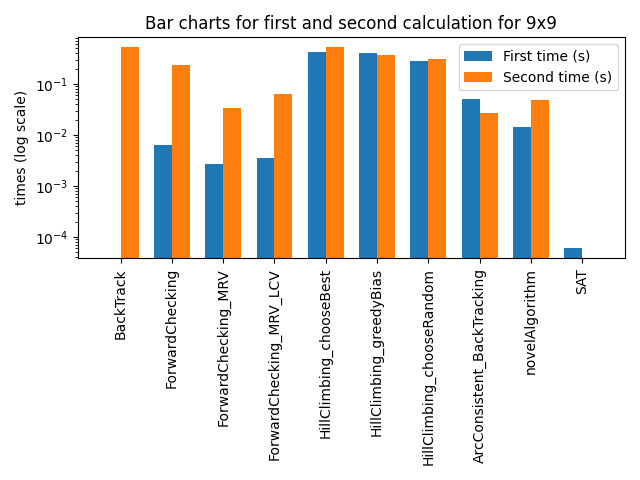
\includegraphics[width=\textwidth]{Pictures/times_9x9}
        \caption{times 9x9}
    \end{subfigure}
    \hfill
    \begin{subfigure}[b]{0.8\textwidth}
        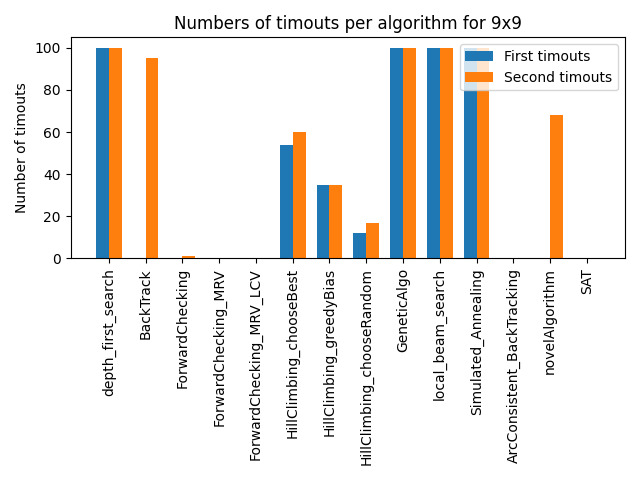
\includegraphics[width=\linewidth]{Pictures/timeouts_9x9}
        \caption{timeouts 9x9}
    \end{subfigure}

    \caption{Comparison of times and timeouts for different solving Algorithms}
\end{figure*}

Wie man unschwer erkennen kann, ist der SAT-Solver mit Abstand am schnellsten und löst die Sudokus innerhalb von meist nicht messbarer Zeit.
Genau gleich sieht es mit den Timeouts aus, bei allen 100 Sudokus hat der SAT-Solver alle Lösungen gefunden. Viele der anderen Solver haben keine einzige Lösung in der gegebenen Zeit gefunden.
Auch wenn sich manche CSP-Lösungsverfahren gut gehalten haben, macht es keinen Sinn etwas anderes als den getesteten SAT-Solver zu verwenden.
Wir können mit ähnlicher Performanz rechnen, da auch cadical-rs so wie die Implementierung in Python auf ersichtlich schnellem Code in C/C++ laufen.

\subsubsection{Implementierung}
Um zu überprüfen ob ein Sudoku eindeutig ist, nutzen wir folgenden Algorithmus~\ref{alg:eindeutig}.
Wenn also durch die Anwendung des Grids auf die Lösungen ein eindeutig lösbares Sudoku entsteht können wir dieses dem Nutzer zurückgeben.
Im Algorithmus~\ref{alg:generierung} wird dargestellt, wie wir hierbei vorgehen.

\begin{algorithm}
    \caption{Sudoku eindeutig lösbar}
    \label{alg:eindeutig}
    \begin{algorithmic}[1]
        \Require $G$ ist ein leeres oder teilweise ausgefülltes $9 \times 9$ Sudoku-Gitter.
        \Require $Solver$ ist eine SAT-Solver mit den entsprechenden Sudoku Klauseln.
        \Ensure Es wird \textbf{true} und die Lösung zurück gegeben wenn das Sudoku eindeutig lösbar ist und \textbf{false} wenn nicht.
        \Function{Eindeutig}{$G, Solver$}
            \State Let $solvable, solution \gets \Call{Solver.solveSudoku}{G}$
            \If{solvable}
                \State $\Call{Solver.prohibitSolution}{solution}$
                \State Let $unique, uniqueSolution \gets \Call{Solver.solveSudoku}{G}$
                \State \Return (unique, $uniqueSolution$)
            \Else
                \State \Return \textbf{false}
            \EndIf
        \EndFunction
    \end{algorithmic}
\end{algorithm}


\begin{algorithm}
    \caption{Sudoku Generierung}
    \label{alg:generierung}
    \begin{algorithmic}[1]
        \Require $G$ ist ein Sudoku-Gitter mit Einsen an markierten und Nullen and unmarkierten Stellen.
        \Require $M$ Menge an vollständigen Sudokus, die wir zur Generierung nutzen.
        \Function{generateSudoku}{$G, M$}
            \State Let $solver \gets \Call{Solver}{G.size}$
            \For{$m \in M$}
                \State Let $transformed \gets G \cdot m$ \Comment{Stellenweise Multiplikation}
                \State Let $unique, solution \gets \Call{Eindeutig}{transformed, solver}$
                \If{$unique$}
                    \State \Return $solution$
                \EndIf
            \EndFor

        \EndFunction
    \end{algorithmic}
\end{algorithm}

Beim Generieren wurden zwei verschiedene Möglichkeiten verglichen, einmal die Generierung ohne und einmal mit Threads.
Das Generieren zu parallelisieren scheint sinnvoll, da es keine großen Abhängigkeiten voneinander gibt.
Die Implementierung mit Threads ist im Grunde die gleiche wie ohne, nur, dass hier die Menge $M$ in die Anzahl von Threads viele disjunktive Teilmengen geteilt wird.
Anschließend wird auf jeder Thread auf einer dieser Teilmengen gestartet. Sobald eine Lösung gefunden wird, werden die anderen Threads unterbrochen.

\subsection{Permutation der Zahlen}
Da alle Lösungsdateien in der ersten Zeile 1 bis 9 geordnet stehen haben, müssen wir die Ziffern in den partiellen Sudokus permutieren.
Beim normalen Markierungsmodus wird die Permutation der Ziffern zufällig gewählt.
Beim Markierungsmodus mit Eingabe von wenigen Ziffern wird die Permutation so gewählt, dass an den markierten Zellen mit Ziffern,
dort auch diese Ziffern stehen.
Dies ist nicht immer möglich bei allen partiellen Sudokus.
Wenn es nicht möglich ist, muss man wieder bei Schritt~\ref{step:fill} anfangen und ein neues partielles Sudoku generieren.


\subsection{Schwierigkeit bewerten}

\subsection{Evaluation}
\begin{table}[h!]
    \centering
    \begin{tabular}{|c|c|c|c|}
        \hline
        \textbf{Anzahl Hinweise} & \textbf{Anzahl true} & \textbf{Anzahl total} & \textbf{Wahrscheinlichkeit} \\
        \hline
        21 & 0     & 3     & 0.00\% \\
        22 & 4     & 147   & 2.72\% \\
        23 & 786   & 1829  & 42.97\% \\
        24 & 10883 & 11879 & 91.62\% \\
        25 & 30508 & 30638 & 99.58\% \\
        26 & 33783 & 33786 & 99.99\% \\
        27 & 16948 & 16948 & 100.00\% \\
        28 & 4235  & 4235  & 100.00\% \\
        29 & 513   & 513   & 100.00\% \\
        30 & 21    & 21    & 100.00\% \\
        31 & 1     & 1     & 100.00\% \\
        \hline
    \end{tabular}
    \caption{Übersicht: Anzahl Hinweise, Anzahl true, Anzahl total und Wahrscheinlichkeit (in Prozent) pro Wert}
\end{table}

\begin{figure}[h!]
    \centering
    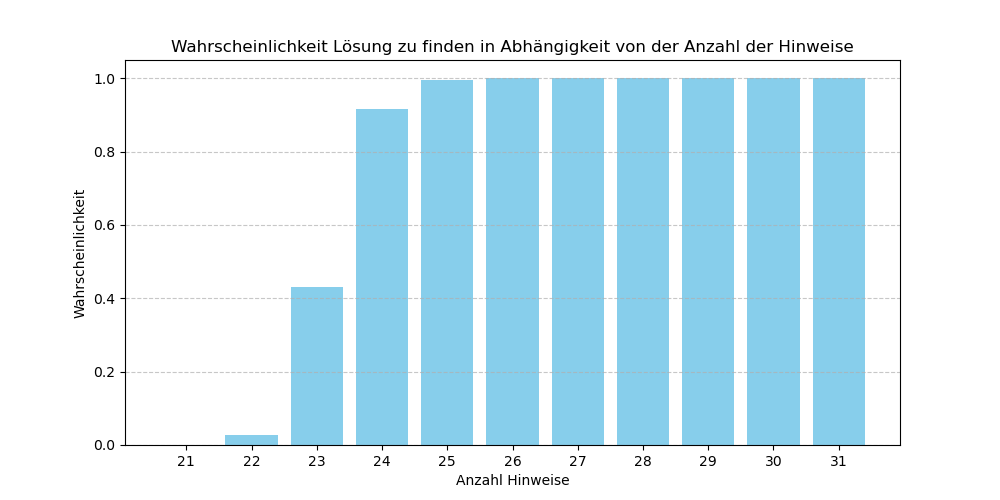
\includegraphics[width=0.8\textwidth]{Pictures/wahrscheinlichkeiten}
    \caption{Wahrscheinlichkeit, dass ein Sudoku mit einer bestimmten Anzahl an Hinweisen eindeutig lösbar ist}
    \label{fig:wahrscheinlichkeiten}

\end{figure}

\begin{figure}[h!]
    \centering
    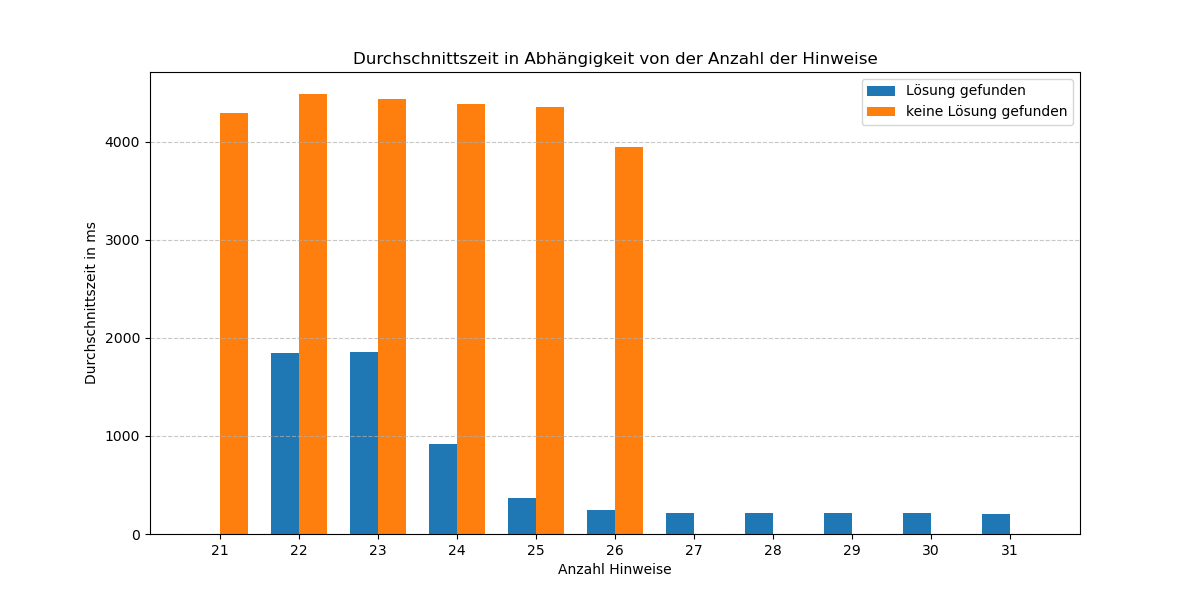
\includegraphics[width=0.8\textwidth]{Pictures/zeiten}
    \caption{Wahrscheinlichkeit, dass ein Sudoku mit einer bestimmten Anzahl an Hinweisen eindeutig lösbar ist}
    \label{fig:zeiten}
\end{figure}

\subsection{Experiment mit CUDA}

Aufgrund der stark parallelen Natur des Problems haben wir ebenfalls einen GPU-basierten Ansatz mithilfe von CUDA untersucht. Dabei wurden sowohl ein CSP- als auch ein SAT-Ansatz implementiert und getestet.
Für Sudokus mit vielen vorgegebenen Hinweisen erzielte die GPU-Lösung vergleichbare Ergebnisse zum CPU-basierten Lösen (Hardware: Nvidia RTX 1050ti vs. AMD Ryzen 7 2700X). Bei Sudokus mit wenigen Vorgaben hingegen schnitt der GPU-Ansatz schlechter ab als die CPU-Lösung.

Dies führen wir insbesondere auf das komplexe \emph{Branching} zurück, welches sich nur bedingt für GPUs eignet. Aufgrund des höheren Aufwands und der geringeren Effizienz haben wir uns letztlich trotz des interessanten Experiments für den CPU-basierten Ansatz entschieden, da dieser einfacher und performanter ist.

\section{Frontend}
\label{sec:frontend}
Das Frontend ist eine Webanwendung, die vollständig im Browser lauffähig ist.
Diese bietet zwei grundlegende Betriebsmodi für die Erstellung von Sudokus an.
Einmal den Markiermodus, in dem Felder visuell hervorgehoben werden können,
und den Eingabemodus, der eine manuelle Eingabe von Zahlen erlaubt.
Die Anwendung unterstützt dabei Sudoku-Größen von 4x4, 6x6 und 9x9.
\\
Die HTML-Datei enthält die grundlegenden Interface-Komponenten der Anwendung. Hierzu gehören:
\begin{itemize}
    \item Schaltflächen zur Auswahl der Sudoku-Größe (4x4, 6x6, 9x9), mit denen dynamisch ein passendes Raster erzeugt wird.
    \item Umschalter zwischen Markier- und Eingabemodus, die das Verhalten der Zellen beim Anklicken verändern.
    \item Das Grid welches beim anklicken verändert werden kann und wo dann bestimmte Muster oder Formen markiert werden können.
    \item Ein Download-Button, der es ermöglicht, das Sudoku als PDF-Datei zu exportieren.
\end{itemize}

Je nach gewählter Sudoku-Größe wird ein entsprechendes Raster dynamisch erzeugt.
Die Zellen erhalten je nach Modus unterschiedliche Eventlistener:
im Markiermodus lassen sie sich an- und abwählen, im Eingabemodus können Zahlen eingegeben werden.
Die Anwendung erlaubt es, zwischen einem Markier- und einem Eingabemodus zu wechseln.
Der aktuelle Modus wird zentral verwaltet, sodass alle Eingabefunktionen sowie Prüfmechanismen entsprechend angepasst sind.
Nach jeder Benutzereingabe wird automatisch überprüft, ob das aktuelle Sudoku gültig ist.
Im Eingabemodus wird dabei auf doppelte Zahlen in Zeilen, Spalten und Blöcken geachtet.
Im Markiermodus wird geprüft, ob genügend Felder markiert sind und ob die Verteilung über das Sudoku-Feld ausreichend ist (mindestens zwei Zeilen und Spalten pro Block müssen belegt sein).
Fehlerhafte Zellen werden visuell hervorgehoben. Die Benutzereingaben werden in ein JSON-Objekt umgewandelt und an eine serverseitige API übermittelt.
Diese verarbeitet das unvollständige Sudoku, berechnet eine mögliche Lösung und sendet sie zurück an den Client.
Die Lösung wird anschließend im dafür vorgesehenen Bereich angezeigt.
\\
Ein besonderes Augenmerk lag bei der Umsetzung auf der Validierung der Sudoku-Regeln.
Dabei musste berücksichtigt werden, dass bei Sudokus der Größen 4x4 und 6x6 die Blockgrößen variieren (2x2 bzw. 2x3).
Die Logik erkennt automatisch die korrekten Blockdimensionen und wendet die Regeln entsprechend an.
Zudem wurde eine eigene Fehlercodierung entwickelt,
um unterschiedliche Arten von Regelverstößen klar voneinander unterscheiden und gezielt anzeigen zu können.
Dazu gehören doppelte Werte, fehlende Verteilung sowie unvollständige Eingaben.
\\
Eine der größten Herausforderungen war die dynamische Erstellung und Validierung unterschiedlich großer Sudoku-Raster sowie die Anpassung der Prüf- und Eingabelogik an zwei Betriebsmodi.
Ebenso anspruchsvoll war die Entwicklung einer robusten Fehlererkennung,
die bei teilweise ausgefüllten Rätseln dennoch konsistente Rückmeldungen geben kann.

\section{Kommunikation}
\label{sec:kommunikation}
\subsection{Kommunikation per POST-Anfrage}

Die Kommunikation zwischen Frontend und Backend erfolgt über POST-Anfragen. Das Frontend sendet dabei Daten im JSON-Format an einen definierten API-Endpunkt des Backends.

\subsection{Frontend-Seite}

Das Frontend erstellt ein JSON-Objekt mit den benötigten Daten und schickt es per POST an das Backend. Beispiel mit JavaScript:

\begin{verbatim}
fetch('/api/endpoint', {
  method: 'POST',
  headers: { 'Content-Type': 'application/json' },
  body: JSON.stringify({ key: 'value' })
})
.then(response => response.json())
.then(data => {
  // Daten verarbeiten und UI aktualisieren
});
\end{verbatim}

\subsection{Backend-Seite}

Das Backend empfängt die POST-Anfrage, liest die JSON-Daten aus, verarbeitet sie (z.B. Validierung, Datenbankzugriff) und sendet eine JSON-Antwort zurück.

\subsection{Antwort}

Die Antwort enthält den Status der Verarbeitung und ggf. weitere Daten im JSON-Format. Das Frontend wertet diese aus und reagiert entsprechend (z.B. Anzeige von Erfolg oder Fehler).

\subsection{Zusammenfassung}

Die Kommunikation basiert auf dem Senden und Empfangen von JSON-Daten per POST-Anfrage. Das Frontend baut die Anfrage, das Backend verarbeitet sie und antwortet mit JSON. So findet der Datenaustausch konkret statt.


\section{Ergebnisse}

\section{Diskussion}

\section{Fazit und Ausblick}

\bibliographystyle{plain}
\bibliography{references}

\appendix
\section{Weitere Graphen}

\end{document}
